\section*{Results}
\subsection*{Summary of model predictive performance}

We used geometric mean abundance (GMA) \cite{santini2017} to quantify site-level alpha diversity, reflecting the richness, abundance and evenness of a sampled species community (normalized to a common 0--1 scale across studies \cite{depalma2021}). For beta diversity, we calculated the Bray-Curtis (BC)\cite{bray1957} compositional similarity between ecologically intact reference sites -- consisting of minimally used primary vegetation -- and sites with other land-use types within the same study\cite{depalma2021}. The resulting GMA and BC distributions are shown in \autoref{fig:response_data_distr}. While GMA can be highest at any site within a study, the BC similarity is capped at reference site levels, which explains the lower mean and thinner tail of the latter distribution. Based on the data distributions, we assumed a beta likelihood function for both alpha and beta diversity models.

%The inflation of zeros was caused by a mix of true absences and imperfect detection\cite{dorazio2016,wu2015}.

Human pressure variables describing land-use \cite{hudson2017}, population density \cite{gpw2017},
and road network density \cite{groads2013} formed the core of all models (see detailed list in \autoref{tab:variables}). In the first model, these constituted the fixed effects, while study-level random intercepts and slopes accounted for inter-study differences in taxonomic scope, environment, and sampling. Spatial block intercepts further captured intra-study variation where available. The model structure, variable selection, and use of generalized linear mixed models largely followed previous implementations \cite{newbold2015,depalma2021,bevan2024,schipper2020}. In the second model, the hierarchical structure consisted of two levels: data was first grouped by biome and high-level taxonomic group, then subdivided by biogeographic realms to form regional biomes\cite{bevan2024} (see \autoref{fig:hierarchical_groups}). Groups containing at least five studies used group-level parameters for predictions, while smaller groups were 'rolled up' to the level above, to avoid overoptimistic performance metrics. Environmental variables included temperature and precipitation\cite{fick2017}, and elevation and slope\cite{amatulli2018} (see \autoref{tab:variables}). Study and block identifiers were included during training to control for study heterogeneity. Here we used a Bayesian hierarchical model to achieve regularization through weakly informative priors, handle overparameterization in small groups, and leverage statistical strength across groups  \cite{dorazio2016,lemoine2019,gelman2006}.

\begin{figure}[H]
    \centering
    \noindent\rule{\linewidth}{0.4pt}\par\vspace{6pt}
    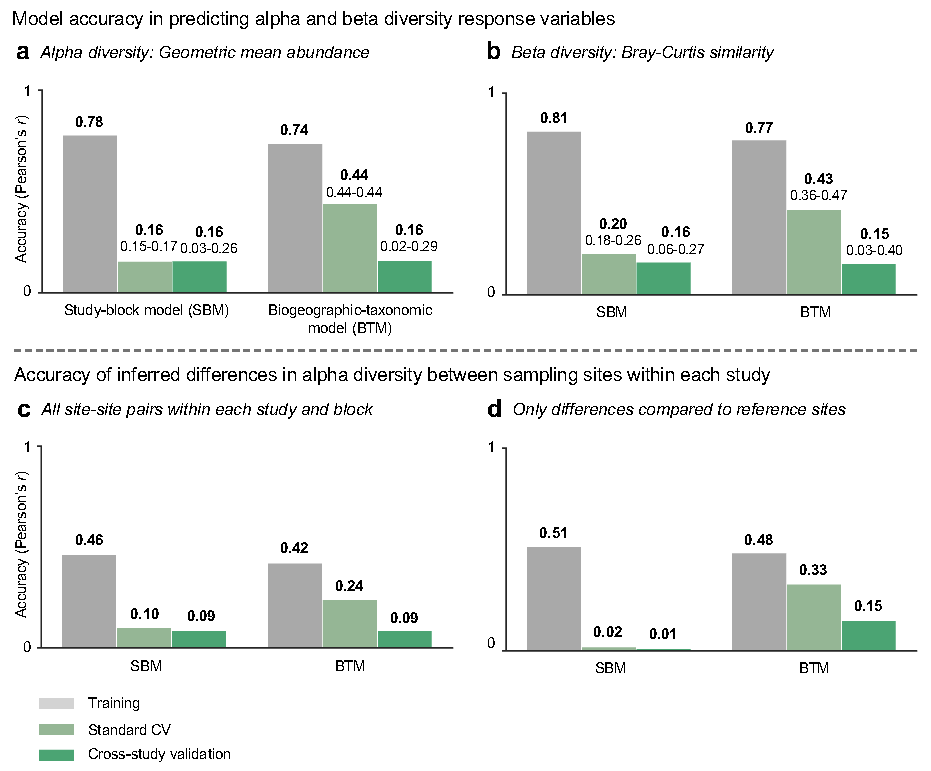
\includegraphics[width=0.95\linewidth]{figures/main/summary_results.pdf}
    \vspace{-10pt}
    \caption{
    \textbf{Summary of model predictive accuracy.}
    \textbf{a–d}, Average predictive accuracy (Pearson's $r$ between predicted and observed values) of the study-block model (SBM) and biogeographic-taxonomic model (BTM). In-sample accuracy on training data is shown in grey, standard cross-validation (CV) accuracy in light green, and cross-study validation accuracy in dark green. For the CV results, the ranges indicate the minimum and maximum accuracies among folds.
    \textbf{a}, Alpha diversity, predictions of site-level geometric mean abundance.
    \textbf{b}, Beta diversity, predictions of Bray–Curtis similarity between pairs of ecologically intact reference sites and other sites, within each study.
    \textbf{c}, Differences in alpha diversity between all site–site pairs within every study and/or block, inferred from the alpha diversity models in (\textbf{a}).
    \textbf{d}, Same as (\textbf{a}) but restricted to pairs containing an ecologically intact reference site.}
    \par\vspace{0pt}\noindent\rule{\linewidth}{0.4pt}
    \vspace{-20pt}
    \label{fig:summary_results}
\end{figure}

A summary of model performance is shown in \autoref{fig:summary_results}. In terms of alpha diversity (\figpanel{fig:summary_results}{a}), the study-block model (SBM, first model above) achieved predictive accuracies of 0.78 on training data, 0.16 in standard cross-validation (CV), and 0.16 in cross-study validation. Accuracy was defined as the Pearson correlation $r$ between observed and predicted values. The corresponding numbers for the biogeographic-taxonomic model (BTM) were 0.74 on training data, 0.44 in standard CV, and 0.16 in cross-study validation. For standard CV, folds were generated using stratified random sampling of \textit{sites} across all studies, to assess generalizability (interpolation accuracy) within sampled contexts. Cross-study validation \cite{bernau2014} evaluated transferability (extrapolation) to other contexts, where each non-overlapping fold contained a stratified random sample of \textit{studies}. For beta diversity (\figpanel{fig:summary_results}{b}) the relative patterns were similar. The accuracies for the SBM were 0.81 (training), 0.20 (standard CV), and 0.16 (cross-study validation); for the BTM they were 0.77, 0.43, and 0.15, respectively. The beta diversity models included the same covariates as described above, plus differences in human population and road density, and the spatial and environmental distance, between sites \cite{depalma2021}. Due to the large number of site pairs in the BC dataset, a sub-sample was used, with inverse weighting based on study size to obtain a more balanced sample.

In addition to the alpha and beta diversity predictions, we looked at estimated and observed \textit{differences} in alpha diversity \textit{within} individual studies and spatial blocks (\figpanel{fig:summary_results}{c,d}), inferred from the predictions in \figpanel{fig:summary_results}{a} (note: these are not separately trained models). The more homogeneous ecological context should provide a more 'level playing field' between the two model structures than \figpanel{fig:summary_results}{a}. When evaluated over all site pairs (\figpanel{fig:summary_results}{c}), the SBM accuracies were at a somewhat lower level than the regular alpha diversity predictions, with standard CV at 0.10 (vs 0.16) and cross-study validation at 0.09 (vs 0.16). The BTM also did worse here, for both standard CV (0.24 vs 0.44) and cross-study validation (0.09 vs 0.16). Finally, we repeated the analysis but restricted to pairs containing reference sites (\figpanel{fig:summary_results}{d}). The inferred site-site differences from the SBM were less accurate than those calculated for all site pairs, yet the opposite was true for the BTM model. It is not clear why that is the case, and since \figpanel{fig:summary_results}{c,d} are not based on a separately trained model, the results should be interpreted with some caution.

\vspace{\baselineskip}

\subsection*{Implications of structural model differences}

The results above reveal notable gaps between in-sample and out-of-sample predictions, with three things standing out: i) The consistently low SBM accuracies; ii) the relatively higher BTM interpolation accuracies (although still quite low in absolute terms); and conversely,  iii) the lack of increase in BTM extrapolation performance. Observation i) is clearly illustrated when comparing the SBM in-sample predictions in \figpanel{fig:lmm_alpha_deepdive}{a} to the out-of-sample results in \figpanel{fig:lmm_alpha_deepdive}{b,c}; predictions were more or less ‘flat’ across all observed values. One key explanation is the low attribution of variance explained\cite{nakagawa2013} to the observable fixed effects (human pressures), relative to the random effects for studies and within-study spatial blocks (\figpanel{fig:lmm_alpha_deepdive}{d}). Since cross-validation simulates model performance on previously unseen sites, the random effects cannot be used when making out-of-sample predictions. The high cross-study heterogeneity around the mean fixed effects (\figpanel{fig:lmm_alpha_deepdive}{e}) further highlights the challenge of model generalization and transferability. Still, as expected from previous studies\cite{keck2025,jaureguiberry2022,newbold2015,depalma2021,bevan2024}, almost all land-use types had negative \textit{average} estimated effects on biodiversity compared to minmally used primary vegetation. The impacts of population and road density were more ambiguous, possibly because these data are static.

The higher BTM interpolation accuracy arose from a combination of model structure -- a biogeographically and taxonomically explicit hierarchy with group-level parameters -- and a richer covariate set. We indeed expect differentiated responses to drivers between groups, and this structure enables generalization of such patterns, assuming that the underlying data is reasonably representative. Further, the richer covariate set was beneficial for predicting alpha diversity across observations globally (\figpanel{fig:summary_results}{a}), where relative distribution patterns depend on environmental factors as well as human pressures, even when data have been normalized. It also helped for beta diversity (\figpanel{fig:summary_results}{b}), since compositional similarity, within the context of a single study, is a function of both human pressures and natural species turnover. The advantage of group-varying parameters also applied when estimating relative levels of alpha diversity within studies and spatial blocks (\figpanel{fig:summary_results}{c,d}). However, there was substantial variation in the average interpolation accuracy between different biogeographic-taxonomic groups, shown for the alpha diversity model in \figpanel{fig:bhm_alpha_groups}{a}, ranging from a few negative values to values close to 0.75. To investigate potential causes of variation, we regressed the group-level accuracies on data attributes of each group (\figpanel{fig:bhm_alpha_groups}{c}). We found that the number of underlying studies and the multivariate Gower distance

\begin{figure}[H]
    \centering
    \noindent\rule{\linewidth}{0.4pt}\par\vspace{6pt}
    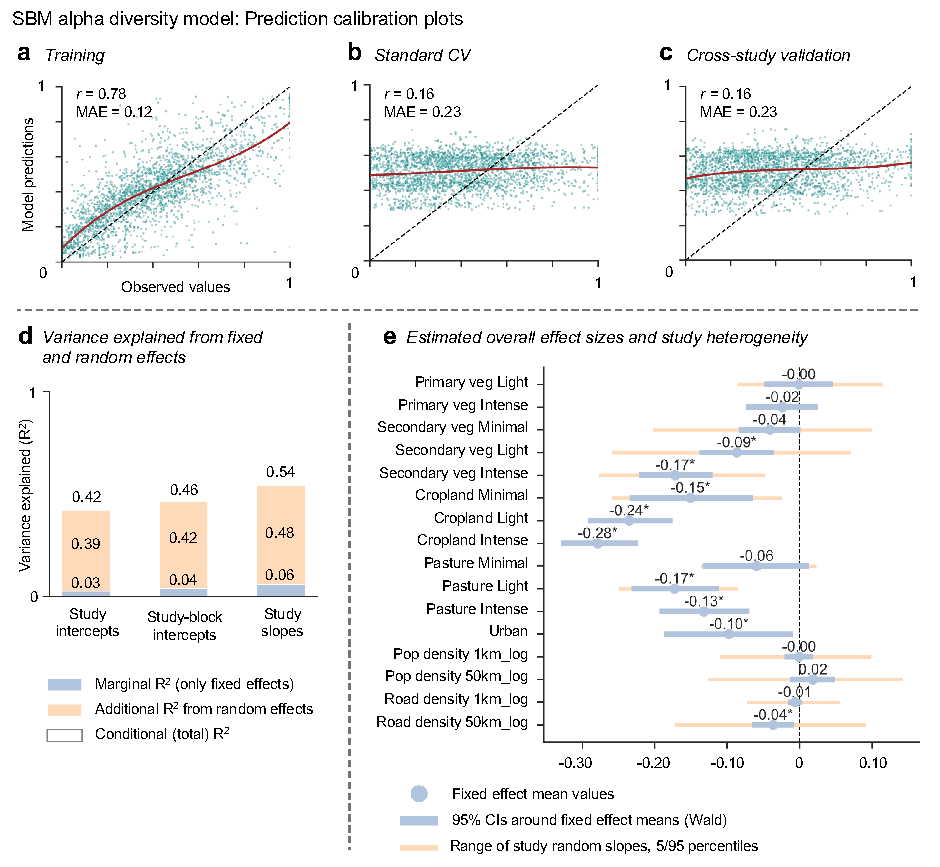
\includegraphics[width=0.95\linewidth]{figures/main/lmm_alpha_deepdive.pdf}
    \vspace{-10pt}
    \caption{
    \textbf{SBM deepdive.}
    \textbf{a}-\textbf{c}, Prediction calibration plots for the SBM alpha diversity model (showing a 10\% random sample for visual clarity), for training data (\textbf{a}), standard CV (\textbf{b}) and cross-study validation (\textbf{c}). The black dashed lines indicate a perfect correlation, whereas the red solid lines show the best polynomial fit to the data.
    %Areas where the solid line is above the dashed line indicate overbiased model predictions, and vice versa.
    \textbf{d}, Decomposition of variance explained between predictions using only the fixed effects (marginal $R^2$, light blue) and predictions including random effects (incremental contribution to conditional $R^2$, yellow). Total variance explained (conditional $R^2$) is shown on top of the bars.
    \textbf{e}, Estimated model parameters. Blue circles show the fixed effect means (across all studies), with blue bars representing 95\% confidence intervals around the mean values. The yellow bars indicate study heterogeneity, the spread of study-level random effects (5–95th percentiles among all studies). Random slope support is uneven across studies, so these estimates are approximate.}
    \par\vspace{0pt}\noindent\rule{\linewidth}{0.4pt}
    \vspace{-20pt}
    \label{fig:lmm_alpha_deepdive}
\end{figure}

between the covariates of each observation and its ten nearest neighbors in the same group, had a negative impact on accuracy (both significant at the 5\% level). This suggests that data heterogeneity negatively impacted performance. On the other hand, the number of taxonomic orders sampled and the standard deviation of the response variable were associated with higher accuracy. One possible interpretation is that the latter captured sampling extensiveness and intensity (together with number of sites, which was positive but not significant), once the aforementioned sources of heterogeneity had been accounted for. However, despite the relative improvement over the SBM, the BTM had clear calibration issues: it overestimated predictions

\begin{figure}[H]
    \centering
    \noindent\rule{\linewidth}{0.4pt}\par\vspace{6pt}
    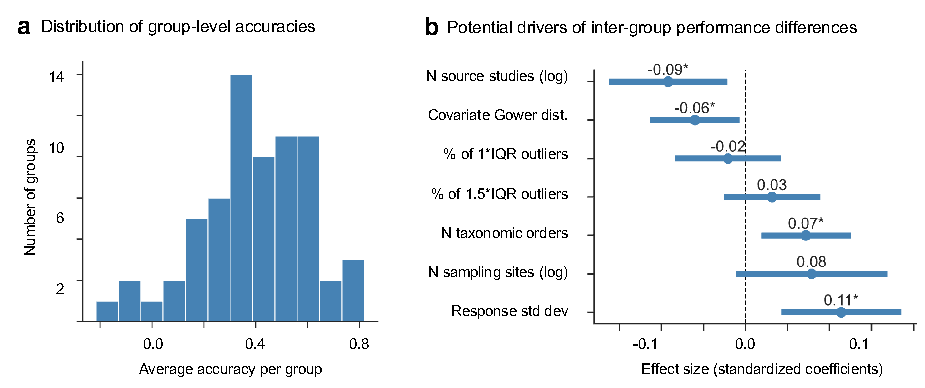
\includegraphics[width=0.95\linewidth]{figures/main/bhm_alpha_groups.pdf}
    \vspace{-10pt}
    \caption{
    \textbf{BTM interpolation deepdive.}
    \textbf{a}, Distribution of group-level average accuracy values of the 60 hierarchical groups included in the BTM model.
    \textbf{b}, Coefficients from linear regression model with group-level accuracy as response variable and data attributes of each group as covariates. All covariates have been standardized to make effect sizes comparable. These should be interpreted as the percentage point change in accuracy from a standard deviation increase in the variable. The bars represent 95\% confidence intervals. The variables are, from top to bottom: The number of source studies in the group (log transformed); the median Gower covariate distance between each observation and its ten nearest neighbors in the same hierarchical group; the proportion of outlier response values (GMA) falling outside of the IQR and 1.5*IQR, respectively; the number of taxonomic orders sampled across studies; the total number of sampling sites (log transformed); the standard deviation of the response variable.
    } \par\vspace{0pt}\noindent\rule{\linewidth}{0.4pt}
    \vspace{-20pt}
    \label{fig:bhm_alpha_groups}
\end{figure}

for small observed values, and vice versa (\figpanel{fig:bhm_alpha_distr_shifts}{b}). This is partially related to the skewness of the response variables (\autoref{fig:response_data_distr}), which is hard to model, but also points to potential bias from latent variables and complex interaction effects.

It should be noted that the structural differences between the models imply some limitations on direct intercomparison. In the SBMs, recall that the fixed effects were estimated based on data from all sites, covering the full spatial and taxonomic scope of the data. The site-level predictions, generated by applying those parameters to local human pressures, were then evaluated against site-level observed values that, naturally, represent a very small share of the full ecological scope of the data. In the absence of taxonomically complete validation data covering major biogeographic regions, this is still a useful approximation. The BTMs, on the other hand, were based on data where the response variables were split by broad taxonomic group. That makes evaluation of predictions more specific to each biogeographic-taxonomic context. While this is a non-negligible difference, it constitutes the best possible way of evaluating the predictions of both models, given the available data.
\vspace{\baselineskip}

\subsection*{Model extrapolation and country-level results}

The drop in BTM extrapolation accuracy (\figpanel{fig:bhm_alpha_distr_shifts}{c}) compared to interpolation (\figpanel{fig:bhm_alpha_distr_shifts}{b}) was caused by distribution shifts between training and test data, which forced the model to make out-of-distribution predictions\cite{meyer2021,meyer2022}. These shifts become evident when comparing the train-test distribution alignment of covariates between the standard CV and cross-study validation runs (\figpanel{fig:bhm_alpha_distr_shifts}{d,e}). Here we calculated the Gower distance \cite{gower1971} between the covariates of each training and test point and its ten nearest neighbors in the training data. The cross-study folds have a higher

\begin{figure}[H]
    \centering
    \noindent\rule{\linewidth}{0.4pt}\par\vspace{6pt}
    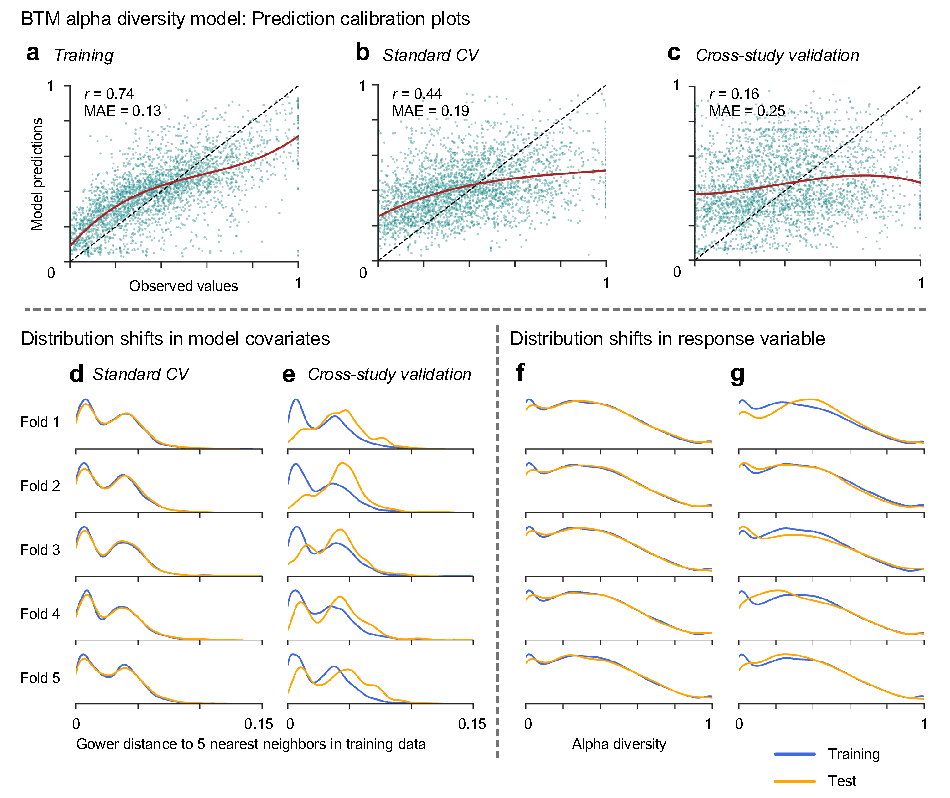
\includegraphics[width=0.95\linewidth]{figures/main/bhm_alpha_distr_shifts.pdf}
    \vspace{-10pt}
    \caption{
    \textbf{BTM extrapolation issues.}
    \textbf{a–c}, Prediction calibration plots for the BTM alpha diversity model (corresponding to the SBM plots in \autoref{fig:lmm_alpha_deepdive}).
    \textbf{d,e}, Distribution density plots obtained by calculating the multivariate Gower distance between the model covariates of each data point, and its hl{five nearest neighbors in the training data (using a sample of 1,000 training points)}. This was done for all training data (blue) and test data (yellow). This gives an indication of how well the joint distribution of covariates align between training and test data in each cross-validation fold, for standard CV (\textbf{d}) and cross-study validation (\textbf{e}).
    \textbf{f,g}, Corresponding density plots of geometric mean abundance of the training and test data in each cross-validation fold, for standard CV (\textbf{f}) and cross-study validation (\textbf{g}).}
    \par\vspace{0pt}\noindent\rule{\linewidth}{0.4pt}
    \vspace{-20pt}
    \label{fig:bhm_alpha_distr_shifts}
\end{figure}

density of test points farther away the training points in covariate space. Some shifts, albeit less pronounced, could be seen for the response variable distributions (\figpanel{fig:bhm_alpha_distr_shifts}{f,g}). At the core, this has to do with model exposure to data. Standard CV involved sampling from a pool of 25,987 sites, such that the model was exposed to a high proportion of the relevant signals in the complete dataset in each fold. In contrast, cross-study validation involved sampling studies from a heterogeneous pool of only 681. This led to a clear spatial, environmental and taxonomic separation of training and test data. Interestingly, although the overall extrapolation accuracies were similar between the two models, the calibration plots (\figrefspanels{fig:lmm_alpha_deepdive}{c}{fig:bhm_alpha_distr_shifts}{c}) show very different patterns. The flexibility of the BTMs, an advantage for interpolation, here led to clear overfitting to the studies seen in training. The SBM, on the other hand, was hampered by the fixed vs random effects issues previously discussed.

The GBF-MF emphasizes country-level reporting of relevant biodiversity indicators \cite{gbfmf2025,affinito2024}. As a complement to the group-level accuracies in \figpanel{fig:bhm_alpha_groups}{b}, we calculated the average accuracy of sampling sites located in each country (\autoref{fig:bhm_country_maps}). We used outputs from the BTM alpha and beta diversity models in the interpolation (standard CV) case. We only included countries with at least two studies and 25 sampling sites, to avoid major outliers skewing the results. The analysis showed large variation in accuracy across countries. This reflects underlying differences in the predictive performance of the models in different biogeographic-taxonomic groups (\figpanel{fig:bhm_alpha_groups}{a}) and the subsets of biogeographic regions, taxa, and sites represented in each country's data (data coverage varies substantially between geographies, see \extfigpanel{fig:predicts_data}{d,e}). Since most country-level datasets are not taxonomically representative, and the need for extrapolation is not factored in, the analysis should be viewed indicatively.

\begin{figure}[tp]
    \centering
    \noindent\rule{\linewidth}{0.4pt}\par\vspace{6pt}
    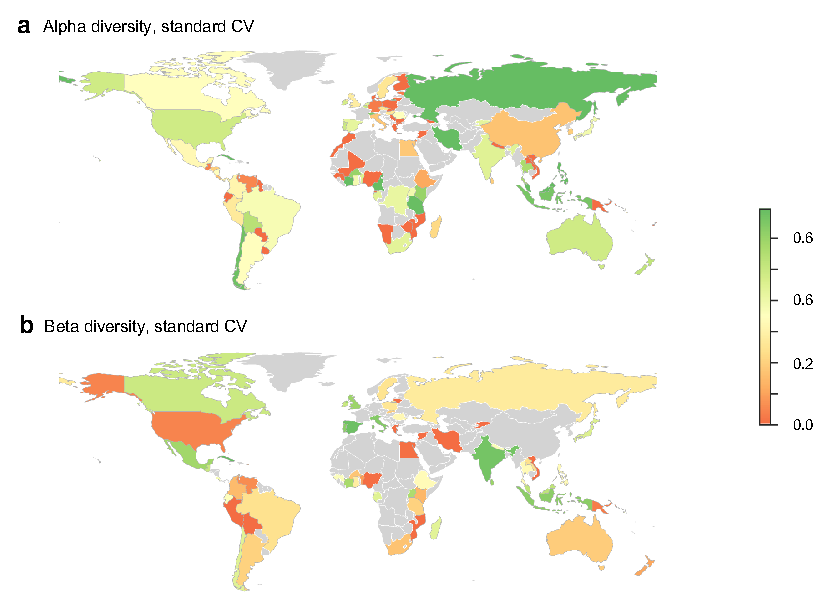
\includegraphics[width=0.95\linewidth]{figures/main/bhm_country_maps.pdf}
    \vspace{-10pt}
    \caption{
    \textbf{BTM accuracy per country.}
    \textbf{a,b}, Average model accuracy calculated per country for the BTM alpha (\textbf{a}) and beta (\textbf{b}) diversity models, when evaluated using standard CV. Only countries with at least two studies and 25 sampling sites are shown. Average accuracy values have been clipped at 0 and winsorized at the 5th and 95th percentiles to prevent outliers from skewing the heatmap gradient. Countries with insufficient data are shown in gray.}
    \par\vspace{0pt}\noindent\rule{\linewidth}{0.4pt}
    \vspace{-20pt}
    \label{fig:bhm_country_maps}
\end{figure}
